\section{Piecewise Linear Model}

The first model, we examined, is a simple piecewise linear function with four discontinuities.
Its discontinuities are at $0, \frac{\pi}{2}, \pi,$ and $\frac{3 \pi}{2}$.
\Cref{equ:pcw.lin.sympi} causes the discontinuities at $0$ and $\pi$ and also the symmetry $f(x + \pi) \equiv f(x) + \pi \mod 2 \pi$.

\begin{align}
    f(x) & = g(x) \mod 2 \pi \label{equ:pcw.lin.f} \\
    g(x) & = \begin{cases}
                 h(x)       & \text{ if } r(x) < \pi \\
                 h(x) + \pi & \text{ else}
             \end{cases} \label{equ:pcw.lin.sympi}
\end{align}

Each arm then is governed by \Cref{equ:pcw.lin.discpihalves}.
It causes the discontinuities at $\frac{\pi}{2}$ and $\frac{3 \pi}{2}$ and also shows the linear nature of the function.
Both parameters $\alpha$ and $\beta$ act here.
$\alpha$ is the slope of the arms and $\beta$ is the offset of the first and third arms.
Examples of how the function looks at different parameter values can be seen in the cobweb diagrams in \Cref{fig:pcw.lin.CobwebA-C}.

\begin{align}
    h(x) & = \begin{cases}
                 \alpha \cdot t(x) + \beta                      & \text{ if } s(x) < \frac{\pi}{2} \\
                 \alpha \cdot t(x) - \alpha \cdot \frac{\pi}{2} & \text{ else}
             \end{cases} \label{equ:pcw.lin.discpihalves}
\end{align}

\Cref{equ:pcw.lin.r,equ:pcw.lin.s} are used to make the above more readable.
They give the modulus of $x$ and some multiple of $\pi$.

\begin{align}
    r(x) & = x \mod 2 \pi \label{equ:pcw.lin.r} \\
    s(x) & = x \mod \pi \label{equ:pcw.lin.s}
\end{align}





\Cref{fig:pcw.lin.2d} shows a bifurcation diagram of the model described above.
The parameter $\beta$ is varied on the interval $[0, 2 \pi]$, because the model will behave the same for $[0, 2 \pi] + k \cdot 2 \pi$.
This is because the result of the function will be taken modulo $2 \pi$ in \Cref{equ:pcw.lin.f}.
The parameter $\alpha$ is varied on the interval $[0, 1]$ because for $\alpha < 0$ nothing especially interesting happens and for $\alpha > 1$ the model shows no periodic behavior.

\begin{figure}
    \centering
    \includegraphics[width=0.7\textwidth]{10_Linear_mod2pi/2D_Period/result.png}
    \caption{2D Bifurcation Diagram of Piecewise Linear Model}
    \label{fig:pcw.lin.2d}
\end{figure}

The two red lines mark the locations of the following one-dimensional scans keeping the parameter $\alpha$ fixed at $0.5$.
\Cref{fig:pcw.lin.1D} shows the scan along the lower red line.
There one can see a period-adding structure.
\Cref{fig:pcw.lin.1DPlusPi} shows the scan along the other red line.
The whole thing is not a period-adding structure, but there is a period-adding structure on the left and on the right of the line in the middle.
Both these structures don't look like period-adding structures normally do.
The interval in the middle of each structure is not the biggest interval with a constant period, but rather some interval that's further to the middle of both structures.

\begin{figure}
    \centering
    \begin{subfigure}{0.4\textwidth}
        \centering
        \includegraphics[width=\textwidth]{10_Linear_mod2pi/1D_Period/result.png}
        \caption{$\beta \in [0.7, 1.7]$}
        \label{fig:pcw.lin.1D}
    \end{subfigure}
    \begin{subfigure}{0.4\textwidth}
        \centering
        \includegraphics[width=\textwidth]{10_Linear_mod2pi/1D_Period_PlusPi/result.png}
        \caption{$\beta \in [3.84, 4.84]$}
        \label{fig:pcw.lin.1DPlusPi}
    \end{subfigure}
    \caption{1D Scans of Piecewise Linear Model showing Periods}
\end{figure}

\Cref{fig:pcw.lin.CobwebA-C} shows a collection of cobwebs diagrams of the three points $P_A$ to $P_C$ marked in \Cref{fig:pcw.lin.1D}.
Note that in this period-doubling structure, all cycles exist in pairs.
At point $P_A$, there are two cycles of period 2 with the symbolic sequences $\A\B$ and $\C\D$ respectively.
When we make the parameter $\beta$ smaller, the cycles move toward the left of the arms.
\Cref{fig:pcw.lin.CobwebA} shows the cycles at the edge of the arms, shortly after that, the cycles collide with the border of the arms.

In the middle interval of \Cref{fig:pcw.lin.1D} with constant period 3, the cycles of $P_A$ are added with the fixed points of the left side.
This Farey-like-adding of cycles is common in period-adding structures~\cite{avrutin2019continuous}.
The fixed points are not shown here but are in the arms $\A$ and $\C$ respectively.
The resulting cycles are $\A^2\B$ and $\C^2\D$ and are shown in \Cref{fig:pcw.lin.CobwebB,fig:pcw.lin.CobwebC}.
These cobweb diagrams also make the movement of the cycles with decreasing parameter $\beta$, mentioned above, clear.
At $P_B$, $\beta$ is bigger and the cycles are at the right edge of the arms.
At $P_C$, the cycles are again at the left edge of the arms.

\begin{figure}
    \centering
    \begin{subfigure}{0.3\textwidth}
        \centering
        \includegraphics[width=\textwidth]{10_Linear_mod2pi/Cobweb_A/result.png}
        \caption{$P_A$}
        \label{fig:pcw.lin.CobwebA}
    \end{subfigure}
    \begin{subfigure}{0.3\textwidth}
        \centering
        \includegraphics[width=\textwidth]{10_Linear_mod2pi/Cobweb_B/result.png}
        \caption{$P_B$}
        \label{fig:pcw.lin.CobwebB}
    \end{subfigure}
    \begin{subfigure}{0.3\textwidth}
        \centering
        \includegraphics[width=\textwidth]{10_Linear_mod2pi/Cobweb_C/result.png}
        \caption{$P_C$}
        \label{fig:pcw.lin.CobwebC}
    \end{subfigure}
    \caption{Cobwebs for first 1D Scan}
    \label{fig:pcw.lin.CobwebA-C}
\end{figure}

\Cref{fig:pcw.lin.CobwebD-F} shows three cobwebs for different points of the second 1D scan in \Cref{fig:pcw.lin.1DPlusPi}.
You can see, that the cycles here do not follow Farey-like-adding like in the other 1D scan.
This is of course because the three cobwebs do not belong to one period adding structure.
The cycles are nonetheless interesting.
The two-cycle at $P_D$, shown in \Cref{fig:pcw.lin.CobwebD}, has the symbolic sequence $\A\C$.
It is on the right edge of the arms at this point and after colliding and skipping the period adding structure, two coexisting cycles appear, shown in \Cref{fig:pcw.lin.CobwebE}.
They have symbolic sequences $\A\D\C$ and $\A\C\B$ respectively.
It is safe to assume, that in the period adding structure between the two points, $P_D$ and $P_E$, the cycles follow Farrey-adding.

\Cref{fig:pcw.lin.CobwebF} shows the 4-cycle at the point $P_F$.
It has the symbolic sequence $\A\D\C\B$ and is at the left edge of the arms.
Lowering the parameter $\beta$ will cause the cycle to collide with the borders and this in turn will lead to the period adding structure we see in the 1D scan in \Cref{fig:pcw.lin.1DPlusPi}.
This period-adding structure will also follow the Farey-like-adding of this cycle and the 3-cycles at point $P_E$, shown in \Cref{fig:pcw.lin.CobwebE}.

\begin{figure}
    \centering
    \begin{subfigure}{0.3\textwidth}
        \centering
        \includegraphics[width=\textwidth]{10_Linear_mod2pi/Cobweb_D/result.png}
        \caption{$P_D$}
        \label{fig:pcw.lin.CobwebD}
    \end{subfigure}
    \begin{subfigure}{0.3\textwidth}
        \centering
        \includegraphics[width=\textwidth]{10_Linear_mod2pi/Cobweb_E/result.png}
        \caption{$P_E$}
        \label{fig:pcw.lin.CobwebE}
    \end{subfigure}
    \begin{subfigure}{0.3\textwidth}
        \centering
        \includegraphics[width=\textwidth]{10_Linear_mod2pi/Cobweb_F/result.png}
        \caption{$P_F$}
        \label{fig:pcw.lin.CobwebF}
    \end{subfigure}
    \caption{Cobwebs for second 1D Scan}
    \label{fig:pcw.lin.CobwebD-F}
\end{figure}
